\documentclass[10pt]{book}
\author{Lan Peng, PhD Student\\ \\Department of Industrial and Systems Engineering\\University at Buffalo, SUNY\\lanpeng@buffalo.edu}
\title{Notes for Operations Research \& More}

\usepackage{amsmath, amssymb, amsthm}
\usepackage{color, soul}
\usepackage[left=1.5cm,right=1.5cm,top=1.5cm,bottom=1.5cm]{geometry}
\usepackage{tabularx}
\usepackage{tikz}
	\usetikzlibrary{shapes.geometric, arrows}
		\tikzstyle{roundedRectangle} = [rectangle, rounded corners, minimum width=3cm, minimum height=1cm,text centered, draw=black]
		\tikzstyle{io} = [trapezium, trapezium left angle=70, trapezium right angle=110, minimum width=3cm, minimum height=1cm, text centered, draw=black]
		\tikzstyle{process} = [rectangle, minimum width=2cm, minimum height=1cm, text centered, draw=black, inner sep=0.1cm]
		\tikzstyle{decision} = [diamond, minimum width=2cm, minimum height=0cm, text centered, draw=black, inner sep=0cm]
		\tikzstyle{arrow} = [thick,->,>=stealth]
		\tikzstyle{circleNode} = [circle, minimum size = 1cm, text centered, draw=black, inner sep=0.1cm]
\usepackage{algorithm}
\usepackage{algorithmic}
\usepackage{bm}
\usepackage{mathrsfs}
\usepackage{hyperref}
\usepackage{longtable}
\usepackage{makecell}
\usepackage{lscape}

\begin{document}
	\maketitle
	\tableofcontents
	\part{Preliminary Topics}
	\chapter{Review of Linear Algebra}

	\chapter{Convex Sets}

	\chapter{Convex Functions and Generalizations}
	\part{Linear Programming}
	\chapter{Formulation}
		\section{Linear Programming Problem Manipulation}
			\subsection{Inequalities and Equalities}
				An inequality can be transformed into an equation by adding or subtracting the nonnegative slack or surplus variable
				\begin{equation}
					\sum_{j=1}^na_{ij}x_j \ge b_i \Rightarrow \sum_{j=1}^na_{ij}x_j - x_{n+1} = b_i 
				\end{equation}
				or
				\begin{equation}
					\sum_{j=1}^na_{ij}x_j \le b_i \Rightarrow \sum_{j=1}^na_{ij}x_j + x_{n+1} = b_i 
				\end{equation}
				Although it is not the practice, equality can be transformed into inequality too
				\begin{equation}
					\sum_{j=1}^na_{ij}x_j = b_i \Rightarrow \begin{cases}\sum_{j=1}^na_{ij}x_j \le b_i \\ \sum_{j=1}^na_{ij}x_j \ge b_i \end{cases} 
				\end{equation}
				Also, in linear programming, we only care about close set, so we will not have $<$, $>$ in the formulation, we can use the following
				\begin{equation}
					\sum_{j=1}^na_{ij}x_j > b_i \Rightarrow \sum_{j=1}^na_{ij}x_j \ge b_i + \epsilon 
				\end{equation}
				where $\epsilon$ is a small number.
			
			\subsection{Minimization and Maximization}
				To convert a minimization problem into a maximization problem, we can use the following to define a new objective function
				\begin{equation}
					\min \sum_{j=1}^nc_jx_j = -\max \sum_{j=1}^n c_jx_j 
				\end{equation}
			
			\subsection{Standard Form and Canonical Form}
				Standard Form
				\begin{align}
					\min \quad & \sum_{j=1}^nc_jx_j \\
					\text{s.t.} \quad & Ax = b \\
									  & x \ge 0 
				\end{align}
				Canonical Form
				\begin{align}
					\min \quad & \sum_{j=1}^nc_jx_j \\
					\text{s.t.} \quad & Ax \le b \\
									  & x \ge 0 
				\end{align}

		\section{Typical Problems}

		\section{Formulation Skills}
			\subsection{Absolute Value}
				Consider the following model statement:
				\begin{align}
					\min \quad & \sum_{j\in J}c_j|x_j|, \quad c_j > 0 \\
					\text{s.t.} \quad & \sum_{j\in J}a_{ij}x_j \gtreqless b_i, \quad \forall i\in I \\
					                  & x_j \quad \text{unrestricted}, \quad \forall j\in J 
				\end{align}
				Modeling:
				\begin{align}
					\min \quad & \sum_{j\in J}c_j(x_j^+ + x_j^-), \quad c_j > 0 \\
					\text{s.t.} \quad & \sum_{j\in J}a_{ij}(x_j^+ - x_j^-) \gtreqless b_i, \quad \forall i\in I \\
					                  & x_j^+, x_j^- \ge 0, \quad \forall j\in J 
				\end{align}

			\subsection{A Minimax Objective}
				Consider the following model statement:
				\begin{align}
					\min \quad & \max_{k\in K}\sum_{j\in J}c_{kj}x_j \\
					\text{s.t.} \quad & \sum_{j\in J}a_{ij}x_j \gtreqless b_i, \quad \forall i\in I \\
					                  & x_j \ge 0, \quad \forall j\in J 
				\end{align}
				Modeling:
				\begin{align}
					\min \quad & z \\
					\text{s.t.} \quad & \sum_{j\in J}a_{ij}x_j \gtreqless b_i, \quad \forall i\in I \\
									  & \sum_{j\in J}c_{kj}x_j \le z, \quad \forall k\in K \\
					                  & x_j \ge 0, \quad \forall j\in J 
				\end{align}
			\subsection{A fractional Objective}
				Consider the following model statement:
				\begin{align}
					\min \quad & \frac{\sum_{j\in J}c_{j}x_j + \alpha}{\sum_{j\in J}d_{j}x_j + \beta} \\
					\text{s.t.} \quad & \sum_{j\in J}a_{ij}x_j \gtreqless b_i, \quad \forall i\in I \\
					                  & x_j \ge 0, \quad \forall j\in J 
				\end{align}
				Modeling:
				\begin{align}
					\min \quad & \sum_{j\in J}c_{j}x_jt + \alpha t \\
					\text{s.t.} \quad & \sum_{j\in J}a_{ij}x_j \gtreqless b_i, \quad \forall i\in I \\
									  & \sum_{j\in J}d_jx_jt + \beta t = 1\\
									  & t > 0 \\
					                  & x_j \ge 0, \quad \forall j\in J \\
					                  & (t = \frac1{\sum_{j\in J}d_jx_j + \beta}) 
				\end{align}
			\subsection{A range Constraint}
				Consider the following model statement:
				\begin{align}
					\min \quad & \sum_{j\in J}c_jx_j \\
					\text{s.t.} \quad & d_i\le \sum_{j\in J}a_{ij}x_j \le e_i, \quad \forall i\in I \\
					                  & x_j \ge 0, \quad \forall j\in J 
				\end{align}
				Modeling:
				\begin{align}
					\min \quad & \sum_{j\in J}c_jx_j, \quad c_j > 0 \\
					\text{s.t.} \quad & u_i + \sum_{j\in J}a_{ij}x_j = e_i, \quad \forall i\in I \\
					                  & x_j \ge 0, \quad \forall j\in J \\
					                  & 0\le u_i \le e_i-d_i, \quad \forall i\in I 
				\end{align}

	\chapter{Simplex Method}
		\section{Basic Feasible Solutions and Extreme Points}
			\begin{definition}
				Consider the system $\{A_{m\times n}x=b_m, x\ge 0\}$, suppose $rank(A, b) = rank(A) =m$, we can arrange $A$ and have a partition of $A$. Let $A=[B, N]$ where $B$ is $m\times m$ invertible matrix, and $N$ is a $m\times (n-m)$ matrix. The solution $x=\left[\begin{matrix}x_B\\x_N\end{matrix}\right]$ to the equation $Ax=b$, where
				\begin{equation}
					x_B = B^{-1}b 
				\end{equation}
				and
				\begin{equation}
					x_N = 0 
				\end{equation}
				is called \textbf{basic solution} of system. If $x_B \ge 0$, it is called \textbf{basic feasible solution}. If $x_B > 0$ it is called \textbf{non-degenerate basic feasible solution}. For $x_B \ge 0$, if some $x_j = 0$, those components are called \textbf{degenerated basic feasible solution}.\\
				$B$ is called the \textbf{basic matrix}, $N$ is called \textbf{nonbasic matrix}				
			\end{definition}

			\begin{theorem}
				$x$ is an E.P. $\iff$ $x$ is a B.F.S
			\end{theorem}
			
			\begin{proof}
				First, Let $x$ be a B.F.S., Suppose $x=\lambda u + (1 - \lambda) v$, for $u, v \in S, \lambda \in (0, 1)$\\
				Let $I = \{i: x_i > 0\}$ Then\\
				- if $i \notin I$ then $x_i = 0$, which implies $u_i = v_i = 0$
				- $\because Au = Av = b$, $\therefore A(u-v) = 0 \Rightarrow \sum_{i=1}^n(u_i - v_i)a_i = 0$, $\because u_i = v_i = 0$, for $i\notin I$, it implies $u_i = v_i$ for $i\in I$, Hence $u=v$, $x$ is E.P.\\
				Second, suppose $x$ is not B.F.S., i.e. $\{a_i: i \in I\}$ are linearly dependent.\\
				Then there $\exists u\ne 0, u_i =0 , i\notin I$ such that $Au=0$.\\
				Hence, for a small $\epsilon$, $x=\frac12(x + \epsilon u) + \frac12(x - \epsilon u)$, $x$ is not E.P.					
			\end{proof}

		\section{Simplex Method}
			\subsection{Key to Simplex Method}
				\subsubsection{Cost Coefficient}
					The cost coefficient can be derived from the following
					\begin{align}
						z &= cx \\
						  &= c_Bx_B + c_Nx_N \\
						  &= c_B(B^{-1}b - B^{-1}Nx_N) + c_Nx_N\\
						  &= c_BB^{-1}b - \sum_{j\in N}(c_BB^{-1}a_j - c_j)x_j \\
						  &= c_BB^{-1}b - \sum_{j\in N}(z_j-c_j)x_j 
 					\end{align}
 					We denote $z_0 = c_BB^{-1}b$, $z_j = c_B^{-1}a_j$, $\bar{b} = B^{-1}b$ and $y_j = B^{-1}a_j$ for all nonbasic variables.\\
 					The formulation can be transformed into
 					\begin{align}
 						\min \quad & z = z_0 - \sum_{j\in N}(z_j - c_j)x_j\\
 						\text{s.t.} \quad & \sum_{j\in N}y_jx_j + x_B = \bar{b} \\
 										  & x_j \ge 0, j\in N \\
 										  & x_B \ge 0 
 					\end{align}
 					In the above formulation, $z_j - c_j$ is the cost coefficient. If $\exists j$ and $z_j - c_j > 0$, it means the objective function can still be optimized. (If $\forall j$, $z_j - c_j \le 0$, then $z \ge z_0$ for any feasible solution, $z$ is the optimal solution)

 				\subsubsection{Pivot}
 					After finding the most violated $z_j - c_j$, we find a variable, say $x_k$, where $z_k - c_k = \min \{z_j - c_j\}$ to be the variable leaving the basis. \\
 					If there are degenerated variables, we can perform different method to choose variable to enter basis.

 				\subsubsection{Minimum Ratio}
 					\begin{equation}
 						x_{B_i} = \bar{b}_i - y_{ik}x_k \ge 0 
 					\end{equation}
 					Therefore we have the minimum ratio rule
 					\begin{equation}
 						x_k = \min_{i \in B} \{\frac{\bar{b}_i}{y_{ik}}, y_{ik} > 0\} 
 					\end{equation}
 					If for the that column all $y_{ik} \le 0$, unbounded.

			\subsection{Simplex Method Algorithm}
				The pseudo-code of Simplex Method is given as following:
				\begin{algorithm}[h!]
					\caption{Simplex Method}
					\begin{algorithmic}[1]
						\REQUIRE Given a basic feasible solution with basis $B$
						\ENSURE Optimal objective value $\min z= cx$
						\STATE Set $\mathbf{B}$ for basic variables, $\mathbf{N}$ for nonbasic variables
						\STATE $\mathbf{B} \gets \text{all slack variables}$
						\STATE $\mathbf{N} \gets \text{all variables excepts slack variables}$
						\FOR{$\forall j$}
							\STATE $z_j=c_BB^{-1}a_j=0$				
						\ENDFOR
						\WHILE{$\exists z_j-c_j > 0$}
							\STATE $z_j=wa_j-c_j=c_BB^{-1}a_j-c_j$
							\STATE $z_k-c_k=\max\limits_{j \in \mathbf{N}}\{z_j-c_j\}$
							\STATE $y_k=B^{-1}a_k$
							\IF{$\exists y_{ik} >0$}
								\STATE $\theta_r=\min\limits_{i \in \mathbf{B}}\{\theta_i=\frac{\bar{b}_i}{y_{ik}}:y_{ik}>0\}$
								\STATE $\mathbf{B} \gets \mathbf{B} \backslash \{k\}$
								\STATE $\mathbf{N} \gets \mathbf{N} \cup \{k\}$
								\STATE $\mathbf{B} \gets \mathbf{B} \cup \{r\}$
								\STATE $\mathbf{N} \gets \mathbf{N} \backslash \{r\}$
							\ELSE
								\STATE Unbounded
							\ENDIF
						\ENDWHILE
						\STATE $x_B^*=B^{-1}b=\bar{b}$
						\STATE $x_N=0$
						\STATE $z^*=c_BB^{-1}b=c_B\bar{b}\mathbf{a_{B_k}}$
					\end{algorithmic}
				\end{algorithm}

		\section{Find Elements in Tableau}
				Initial tableau:\\
				\begin{align}
					\begin{tabular} {|c|c|c|c|c|c|c|c|}
						\hline
						& $z$ & $x_1$ & $x_2$ & $x_3$ & $x_4$ & $x_5$ & RHS \\
						\hline
						$z$ & 1 & 1 & 3 & 0 & 0 & 0 & 0 \\
						\hline
						$x_3$ & 0 & 1 & -2 & 1 & 0 & 0 & 0 \\
						\hline
						$x_4$ & 0 & -2 & \framebox{1} & 0 & 1 & 0 & 4\\
						\hline
						$x_5$ & 0 & 5 & 3 & 0 & 0 & 1 & 15 \\
						\hline
					\end{tabular}
				\end{align}
				Last tableau:\\
				\begin{align}
					\begin{tabular} {|c|c|c|c|c|c|c|c|}
						\hline
						& $z$ & $x_1$ & $x_2$ & $x_3$ & $x_4$ & $x_5$ & RHS \\
						\hline
						$z$ & 1 & 0 & 0 & 0 & $-\frac{12}{11}$ & $-\frac{7}{11}$ & $-\frac{153}{11}$ \\
						\hline
						$x_3$ & 0 & 0 & 1 & 1 & $\frac{13}{11}$ & $\frac{3}{11}$ & $\frac{97}{11}$ \\
						\hline
						$x_2$ & 0 & 1 & 0 & 0 & $\frac{5}{11}$ & $\frac{2}{11}$ & $\frac{50}{11}$ \\
						\hline
						$x_1$ & 1 & 0 & 0 & 0 & $-\frac{3}{11}$ & $\frac{1}{11}$ & $\frac{3}{11}$ \\
						\hline
					\end{tabular}
				\end{align}
				- The optimal basic variables are $x_3$, $x_2$, $x_1$. The optimal basis is the columns in the initial tableau with correspond columns
				\begin{equation}
					B = \left(\begin{matrix}
						\frac{13}{11} & \frac{3}{11} & \frac{97}{11}\\
						\frac{5}{11} & \frac{2}{11} & \frac{50}{11}\\
						-\frac{3}{11} & \frac{1}{11} & \frac{3}{11}\\
					\end{matrix}\right)
				\end{equation}
				- From the initial tableau, we can see the initial basis is built from slack variables $x_3$, $x_4$, $x_5$. The $B^{-1}$ is the correspond columns in final tableau.
				\begin{equation}
					B = \left(\begin{matrix}
						1 & -2 & 1\\
						0 & 1 & -2\\
						0 & 3 & 5\\
					\end{matrix}\right) 		
				\end{equation}
				- The optimal basic variables are $x_3$, $x_2$, $x_1$. Find $c_B$ in the initial tableau.
				\begin{equation}
					c_B = \left(\begin{matrix}
						0\\3\\1
					\end{matrix}\right) 
				\end{equation}
				- Find $w=c_BB^{-1}$ from the final tableau, correspond to the slack variable.
				\begin{equation}
					w = c_BB^{-1} = \left(\begin{matrix}
						0\\-\frac{12}{11}\\-\frac7{11}
					\end{matrix}\right) 
				\end{equation}

		\section{Artificial Variable}
			If some of the constraint is not in $\sum_{i=1}^na_ix_i \le 0$ form, we cannot add a positive slack variable. In this case, we add an artificial variable other than slack variable.
			\begin{equation}
				\sum_{i=1}^n a_ix_i \ge (or =) 0 \Rightarrow \sum_{j=1}^n a_ix_i + x_a = 0 
			\end{equation}
			Notice that in an optimal solution, $x_a = 0$, otherwise it is not valid.\\
			Artificial variables are only a tool to get the simplex method started.
			\subsection{Two-Phase Method}
				\subsubsection{Two-Phase Method}
					For \textbf{Phase I:}\\
						Solve the following program start with a basic feasible solution $x=0, x_a=b$, i.e., the artificial variable forms the basis.
						\begin{align}
							\min \quad & 1x_a \\
							\text{s.t.} \quad & Ax + x_a = b \\
											  & x \ge 0 \\
											  & x_a \ge 0 
						\end{align}
						If the optimal $1x_a \ne 0$, infeasible, stop. Otherwise proceed Phase II.
					For \textbf{Phase II:}\\
						Remove the columns of artificial variables, replace the objective function with the original objective function, proceed to solve simplex method.
				\subsubsection{Discussion}
					\textbf{Case A:} $x_a \ne 0$\\
						Infeasible.\\
					\textbf{Case B.1:} $x_a = 0$ and all artificial variables are out of the basis\\
					At the end of Phase I, we derive
					\begin{align}
						\begin{tabular} {|c|c|c|c|c|}
							\hline
							$x_0$ & $x_B$ & $x_N$ & $x_a$ & RHS \\
							\hline
							1 & 0 & 0 & -1 & 0\\
							\hline
							0 & $I$ & $B^{-1}N$ & $B^{-1}$ & $B^{-1}b$ \\
							\hline
						\end{tabular} 
					\end{align}
					We can discard $x_a$ columns, (or we can leave it because it keeps track of $B^{-1}$), and then we do the Phase II
					\begin{align}
						\begin{tabular} {|c|c|c|c|}
							\hline
							$z$ & $x_B$ & $x_N$ & $RHS$ \\
							\hline
							1 & 0 & $c_BB^{-1}N - c_N$ & $c_BB^{-1}b$ \\
							\hline
							0 & $I$ & $B^{-1}N$ & $B^{-1}b$ \\
							\hline
						\end{tabular} 		
					\end{align}
					\textbf{Case B.2:} Some artificial variables are in the basis at zero values\\
					This is because of degeneracy. We pivot on those artificial variables, once they leave the basis, eliminate them.
			\subsection{Big M Method}

			\subsection{Single Artificial Variable}

		\section{Revised Simplex Method}
			\subsection{Key to Revised Simplex Method}
				The procedure of Simplex Method is (almost) exactly the same as original simplex method. However, notice that we don't need to use $N$ so for the revised simplex method, we don't calculate any matrix related to $N$\\
				The original matrix:
				\begin{align}
					\begin{tabular} {|c|c|c|c|}
						\hline
						$z$ & $x_B$ & $x_N$ & $RHS$ \\
						\hline
						1 & 0 & $c_BB^{-1}N - c_N$ & $c_BB^{-1}b$ \\
						\hline
						0 & $I$ & $B^{-1}N$ & $B^{-1}b$ \\
						\hline
					\end{tabular} 		
				\end{align}
				The revised matrix:
				\begin{align}
					\begin{tabular} {|c|c|}
						\hline
						Basic Inverse & RHS \\
						\hline
						$w=c_BB^{-1}$ & $c_B\bar{b} = c_BB^{-1}b$\\
						\hline
						$B^{-1}$ & $\bar{b} = B^{-1}b$\\
						\hline
					\end{tabular} 
				\end{align}
				For each pivot iteration, calculate $z_j - c_j = wa_j - c_j = c_BB^{-1}a_j - c_j, \forall j\in N$, pivot rules are the same as simplex method, each time find a variable $x_k$ to enter basis
				\begin{align}
					\begin{tabular}{|c|c|c|c|}
						\cline{1-2} \cline{4-4} $B^{-1}$ & RHS & & $x_k$ \\
						\cline{1-2} \cline{4-4} $w$ & $c_B\bar{b}$ & & $z_k-c_k$ \\
						\cline{1-2} \cline{4-4} $B^{-1}$ & $\bar{b}$ & & $y_k$ \\
						\cline{1-2} \cline{4-4}
					\end{tabular} 
				\end{align}
				Do the minimum ratio rule to find the variable $x_r$ to leave the basis
				\begin{align}
					\begin{tabular}{|c|c|c|c|}
						\cline{1-2} \cline{4-4} $B^{-1}$ & RHS & & $x_k$ \\
						\cline{1-2} \cline{4-4} $w$ & $c_B\bar{b}$ & & $z_k-c_k$ \\
						\cline{1-2} \cline{4-4} & $\bar{b_1}$ & & $y_{1k}$\\
						& $\bar{b_2}$ & & $y_{2k}$\\
						& ... & & ...\\
						$B^{-1}$ & $\bar{b_r}$ & & $y_{rk}$(pivot at here)\\
						& ... & & ...\\
						& $\bar{b_m}$ & & $y_{mk}$\\
						\cline{1-2} \cline{4-4} 
					\end{tabular}
				\end{align}

			\subsection{Comparison between Simplex and Revised Simplex}
				\subsubsection{Advantage of Revised Simplex}
				- Save storage memory \\
				- Don\rq{}t need to calculate N (including $B^{-1}N$ and $c_BB^{-1}N$) \\
				- More accurate because round up errors will not be accumulated 

				\subsubsection{Disadvantage of Revised Simplex}
				- Need to calculate $wa_j$ for all $j \in N$ (in fact don\rq{}t need to calculated it for the variable just left the basis) 

				\subsubsection{Computation Complexity}
				\begin{align}
					\begin{tabular}{|c|c|c|}
						\hline Method & Type & Operations\\
						\hline Simplex & $\times$ & $(m+1)(n-m+1)$\\
						\cline{2-3} & $+$ & $m(n-m+1)$\\
						\hline Revised Simplex & $\times$ & $(m+1)^2+m(n-m)$ \\
						\cline{2-3} & $+$ & $m(m+1)+m(n-m)$ \\
						\hline
					\end{tabular} 
				\end{align}

				\subsubsection{When to use?}
				- When $m >> n$, do revise simplex method on the dual problem \\
				- When $m \simeq n$, revise simplex method is not as good as simplex method \\
				- When $m << n$ perfect for revise simplex method.
				
			\subsection{Decomposition of B inverse}
				Let $B=\{ a_{B_1}, a_{B_2}, ..., a_{B_r}, ..., a_{B_m}\}$ and $B^{-1}$ is known.
				If $a_{B_r}$ is replaced by $a_{B_k}$, then $B$ becomes $\bar{B}$. Which means $a_{B_r}$ enters the basis and $a_{B_k}$ leaves the basis. \\
				Then $\bar{B}^{-1}$ can be represent by $B^{-1}$. Noting that $a_k=By_k$ and $a_{B_i}=Be_i$, then
				\begin{align}
					\bar{B} & = (a_{B_1}, a_{B_2}, ...,a_{B_{r-1}}, a_k, a_{B_{r+1}}, a_m)  \\
					& = (Be_1, Be_2, ..., Be_{r-1}, By_k, Be_{r+1}, ..., Be_m)  \\
					& = BT 
				\end{align}
				where $T$ is
				\begin{equation}
					T=\left[ \begin{array}{cccccccc}
						1 & 0 & ... & 0 & y_{1k} & 0 & ... & 0 \\
						0 & 1 & ... & 0 &  y_{2k} & 0 & ... & 0 \\
						\vdots & \vdots & & \vdots & \vdots & \vdots & & \vdots \\
						0 & 0 & ... & 1 & y_{r-1,k} & 0 & ... & 0 \\
						0 & 0 & ... & 0 & y_{rk} & 0 & ... & 0 \\
						0 & 0 & ... & 0 &  y_{r+1,k} & 1 & ... & 0 \\
						\vdots & \vdots & & \vdots & \vdots & \vdots & & \vdots \\
						0 & 0 & ... & 0 &  y_{mk}& 0 & ... & 1 \\
					\end{array} \right] 
				\end{equation}
				and 
				\begin{equation}
					E =  T ^{-1}=\left[ \begin{array}{cccccccc}
						1 & 0 & ... & 0 & \frac{-y_{1k}}{y_{rk}} & 0 & ... & 0 \\
						0 & 1 & ... & 0 & \frac{-y_{2k}}{y_{rk}} & 0 & ... & 0 \\
						\vdots & \vdots & & \vdots & \vdots & \vdots & & \vdots \\
						0 & 0 & ... & 1 & \frac{-y_{r-1,k}}{y_{rk}} & 0 & ... & 0 \\
						0 & 0 & ... & 0 & \frac{1}{y_{rk}} & 0 & ... & 0 \\
						0 & 0 & ... & 0 & \frac{-y_{r+1,k}}{y_{rk}} & 1 & ... & 0 \\
						\vdots & \vdots & & \vdots & \vdots & \vdots & & \vdots \\
						0 & 0 & ... & 0 &  \frac{-y_{mk}}{y_{rk}} & 0 & ... & 1 \\
					\end{array} \right] 
				\end{equation}
				For each iteration, i.e. one variable enters the basis and one leaves the basis, $\bar{B}^{-1}=T^{-1}B^{-1}=EB^{-1}$. Given that the first iteration starts from slack variables, the first basis $B_1$ is $I$, then we have
				\begin{equation}
					B^{-1}_t=E_{t-1} E_{t-2} \cdots E_{2} E_{1} I
				\end{equation}
				Using $E$ in calculation can simplify the product of matrix where
				\begin{align}
					cE &= {c_1,c_2,...,c_m} \left[ \begin{array}{cccccc}
					1 & 0 & ... & g_1 & ... & 0 \\
					0 & 1 & ... & g_2 & ... & 0 \\
					\vdots & \vdots & & \vdots & & \vdots \\
					0 & 0 & ... & g_m & ... & 1 \\
					\end{array} \right]  \\
					&= (c_1, c_2, ... ,c_{r-1}, cg, c_{r+1}, ..., c_m) 
				\end{align}
				and
				\begin{align}
					Ea &=  \left[ \begin{array}{cccccc}
					1 & 0 & ... & g_1 & ... & 0 \\
					0 & 1 & ... & g_2 & ... & 0 \\
					\vdots & \vdots & & \vdots & & \vdots \\
					0 & 0 & ... & g_m & ... & 1 \\
					\end{array} \right]
					 \left[ \begin{array}{c}
					a_1 \\
					a_2 \\
					\vdots \\
					a_m \\
					\end{array} \right]  \\
					&= 
					\left[ \begin{array}{c}
					a_1 \\
					a_2 \\
					\vdots \\
					a_{r-1} \\
					0 \\
					a_{r+1} \\
					\vdots \\
					a_m \\
					\end{array} \right] +
					a_r\left[ \begin{array}{c}
					g_1 \\
					g_2 \\
					\vdots \\
					g_{r-1} \\
					g_r \\
					g_{r+1} \\
					\vdots \\
					g_m \\
					\end{array} \right]  \\
					&=\bar{a}+a_rg 
				\end{align}
				Then we can calculate $w$, $y_k$ and $\bar{b}$
				\begin{align}
					w&=c_BB^{-1} = c_BE_{t-1}E_{t-2}...E_2E_1  \\
					y_k &=B^{-1}a_k = E_{t-1}E_{t-2}...E_2E_1a_k  \\
					\bar{b}&=B^{-1}_{t+1}b=E_tE_{t-1}E_{t-2}...E_2E_1b 
				\end{align}

		\section{Simplex for Bounded Variables}
			\subsection{Bounded Variable Formulation}
				\begin{align}
					\min \quad & cx \\
					\text{s.t.} \quad & Ax=b \\
									  & l \le x\le b 
				\end{align}
				Reason why we don't the following formulation
				\begin{align}
					\min \quad & cx \\
					\text{s.t.} \quad & Ax=b \\
					                  & x - Ix_l = l \\
					                  & x + Ix_u = u \\
					                  & x \ge 0\\
					                  & x_l \ge 0\\
					                  & x_u \ge 0 
				\end{align}
				is that this formulation increase the number of variable from $n$ to $3n$, and the number of constraint from $m$ to $m+2n$, the size in increase significantly.

			\subsection{Basic Feasible Solution}
				Consider the system $Ax=b$ and $l\le x\le b$, where $A$ is a $m\times n$ matrix of rank $m$, the solution $\bar{x}$ is a \textbf{basic feasible solution} if $A$ can be partition into $[B, N_l, N_u]$ where the solution $x$ can be partition into $x=(x_B, x_{N_l}, x_{N_u})$, in which $\bar{x}_{N_l} = l_{N_l}$ and $\bar{x}_{N_u} = u_{N_u}$, therefore
				\begin{equation}
					\bar{x}_B = B^{-1}b - B^{-1}N_lx_{N_l} - B^{-1}N_ux_{N_u} 
				\end{equation}
				Furthermore, similar to definition of nonnegative variables, if $l_B \le x_B \le u_B$, $x_B$ is a basic feasible solution, if $l_B < x_B < u_B$, $x_B$ is a non-degenerate basic feasible solution. 

			\subsection{Improving Basic Feasible Solution}
				The basic variables and the objective function can be derived as following:
				\begin{align}
					x_B &= B^{-1}b - B^{-1}N_lx_{N_l} - B^{-1}N_ux_{N_u} \\
					  z &= c_Bx_B + c_{N_l}x_{N_l} + c_{N_u}x_{N_u} \\
					  	&= c_B(B^{-1}b - B^{-1}N_lx_{N_l} - B^{-1}N_ux_{N_u})  \\
					  	& \quad + c_Bx_B + c_{N_l}x_{N_l} + c_{N_u}x_{N_u}\\
					  	&= c_BB^{-1}b + (c_{N_l} - c_BB^{-1}N_l)x_{N_l} \\
					  	& \quad + (c_{N_u} - c_BB^{-1}N_u)x_{N_u} \\
					  	&= c_BB^{-1}b - \sum_{j \in J_1}(z_j - c_j)x_j - \sum_{j \in J_2}(z_j - c_j)x_j
				\end{align}
				$J_1$ is the set of variables at lower bound, $J_2$ is the set of the variables at upper bound.\\
				Notice that the right-hand-side no longer provide $c_BB^{-1}b$ and $B^{-1}b$. For the variable entering the basis, find the variable with
				\begin{equation}
					\max\{\max_{j\in J_1}\{z_j - c_j\}, \max_{j\in J_2}\{c_j - z_j\}\} 
				\end{equation}
				to enter the basis\\
				\framebox{\textbf{Tip:}} "Most violated rule"\\
				The minimum ratio rule is revised for bounded simplex
				\begin{align}
					\Delta &= \min \{\gamma_1, \gamma_2, u_k-l_k\} \\
					\gamma_1 &= \begin{cases}
									\min_{r\in J_1}\{\frac{\bar{b}_r-l_{B_r}}{y_{rk}}:y_{rk} > 0\} \\
									\min_{r\in J_2}\{\frac{\bar{b}_r-l_{B_r}}{-y_{rk}}:y_{rk} < 0\} \\
									\infty
								\end{cases} \\
					\gamma_2 &= \begin{cases}
									\min_{r\in J_1}\{\frac{u_{B_r} - \bar{b}_r}{-y_{rk}}:y_{rk} < 0\} \\
									\min_{r\in J_2}\{\frac{u_{B_r} - \bar{b}_r}{y_{rk}}:y_{rk} > 0\} \\
									\infty
								\end{cases} 
				\end{align}
				\framebox{\textbf{Tip:}}\\
				Use $l \le x+\Delta \le u$ to test the range of $\delta$, if it hits lower bound, it is called $\gamma_1$, if it hits upper bound, it is called $\gamma_2$.

		\section{Degeneracy and Cycling}
			\subsection{Degeneracy}
				\subsubsection{Degeneracy in Simplex Method}
					If the basic variable $x_B$ is not strictly $> 0$, i.e. if some basic variable equals to 0, we call it degenerate.

				\subsubsection{Degeneracy for Bounded Variables}
					If some basic variables are at their upper bound or lower bound, we call it degenerate.

			\subsection{Cycling}
				In the degenerate case, pivoting by the simplex rule does not always give a strict decrease in the objective function value, because it may have $b_r = 0$. It is possible that the tableau may repeat if we use the simplex rule.\\
				Geometrically speaking, it means that at the same point - extreme point - it corresponds to more than one feasible solutions, so when we are pivoting, we stays at the same place.\\
				In computer algorithm, we rarely care about cycling because the data in computer is not precise, it is very hard to get into cycling.

			\subsection{Cycling Prevent}
				\subsubsection{Lexicographic Rule}
					- For entering variable, same as simplex rule\\
					- For leaving variable, if there is a tie, choose the variable with the smallest $\frac{y_{r1}}{y_{rk}}$.

				\subsubsection{Bland's Rule}
					- For entering variable, choose the variable with smallest index where $z_j - c_j \le 0$\\
					- For leaving variable, if there is a tie, choose the variable with smallest index.

				\subsubsection{Successive Ratio Rule}
					- Select the pivot column as any column $k$ where $z_k - c_k \le 0$\\
					- Given $k$, select the pivot row $r$ as the minimum successive ratio row associated with column $k$.\\
					In other words, for pivot columns where there is no tie in the usual minimum ratio, the successive ratio rule reduces to the simplex rule

		\section{Dual Simplex Method}
			Maintain dual feasibility, i.e. primal optimality, and complementary slackness and work towards primal feasibility.
			\framebox{\textbf{Tip:}}The RHS become new $z_j - c_j$, the old $z_j - c_j$ become new RHS. We are actually solving the dual problem.

		\section{As a Search Algorithm}
			\subsection{Improving Search Algorithm}
				A simplex method is a search algorithm, for each iteration it finds a not-worse solution, which can be represented as:\\
				\begin{equation}x^t = x^{t-1}+\lambda_{t-1}d^{t-1}  \end{equation}
				Where\\
				- $x^t$ is the solution of the $t$th iteration\\
				- $\lambda_t$ is the step length of $t$th iteration\\
				- $d^t$ is the direction of the $t$th iteration\\
				For each iteration, it contains three steps:\\
				- Optimality test\\
				- Find direction\\
				- Find the step length
				
			\subsection{Optimality Test}
				\begin{align}
					z &= cx \\
					& = \left[\begin{matrix}c_B & c_N\end{matrix} \right] \left [ \begin{matrix}x_B \\ x_N \end{matrix} \right]  \\
					& = c_B x_B + c_N x_N  \\
				\text{and} \because &Ax=b  \\
					\therefore & Bx_B + Nx_N = b, x_B\ge 0, x_N\ge 0 \\
					\therefore & x_B = B^{-1}b-B^{-1}Nx_N \\
					z &= c_BB^{-1}b-c_BB^{-1}Nx_N+c_Nx_N
				\end{align}
				for current solution $\hat{x}=\left [\begin{matrix}\hat{x_B} \\ 0\end{matrix}\right]$, $\hat{z} = c_BB^{-1}b$, then
				\begin{equation}
					z - \hat{z} = \left[\begin{matrix}0 & c_N - c_BB^{-1}N \end{matrix} \right] \left[ \begin{matrix}x_B \\ x_N \end{matrix}\right] 
				\end{equation}
				The $c_N - c_BB^{-1}N$ is the reduced cost, for a minimized problem, if $c_N - c_BB^{-1}N > 0$ means $z - \hat{z} \ge 0$, it reaches the optimality because we cannot find a solution less than $\hat{z}$.\\
							
			\subsection{Find Direction}
				Suppose we choose $x_k$ as a candidate to pivot into Basis\\
				\begin{equation}
					x = \left[ \begin{matrix}B^{-1}b-B^{-1}a_kx_k \\ 0+e_kx_k\end{matrix}\right]=\left[ \begin{matrix}B^{-1}b \\ 0\end{matrix} \right] + \left[ \begin{matrix} -B^{-1}a_k \\ e_k \end{matrix} \right]x_k 
				\end{equation}
				In this form, we can see: $x$ is the result after $t$th iteration, $\left[ \begin{matrix}B^{-1}b \\ 0\end{matrix} \right]$ is the result after $(t-1)$th iteration. $ \left[ \begin{matrix} -B^{-1}a_k \\ e_k \end{matrix} \right]$ is the iteration direction, $x_k$ is the step length.\\
				The only requirement of $x_k$ is $r_k < 0$ where $r_k=c_k - z_k$ is reduce cost, which is the $k$th entry of $c_N - c_BB^{-1}N$. \\
				Generally speaking, we usually take $r_k = \min\{c_j - z_j\}$ (which in fact can not guarantee the efficient of the algorithm.)

			\subsection{Find the Step Length}
				We need to guarantee the non-negativity, so for each iteration, we need to make sure $x\ge 0$. Which means\\
				\begin{equation}B^{-1}b-B^{-1}a_kx_k \ge 0  \end{equation}
				Denote $B^{-1}b$ as $\bar{b}$, denote $B^{-1}a_k$ as $y_k$\\
				If $y_k \le 0$, we can have $x_k$ as large as infinite, which means unboundedness. \\
				If $y_k > 0$ now we can use the minimum ratio to guarantee non-negativity.\\
				\textbf{Remember} hit the bound, basic variable leave the basis and become non-basic variable.
			\subsection{Simplex Method Algorithm}

			\subsection{Simplex Method Tableau}

			\subsection{Simplex Method as a Search Algorithm}

	\chapter{Duality, Sensitivity and Relaxation}
		\section{Duality}
			\subsection{Dual Formulation}
				For any prime problem
				\begin{align}
					\text{min} \quad & cx \\
					\text{s.t.} \quad & Ax\ge b \\
								& x\ge 0 
				\end{align}
				we can have a dual problem
				\begin{align}
					\text{max} \quad & wb  \\
					\text{s.t.} \quad & wA\le c\\
								& w \ge 0
				\end{align}
				
			\subsection{Mixed Forms of Duality}
				For the following prime problem
				\begin{align}
					\text{P(or D)} \quad \min \quad & c_1x_1 + c_2x_2 + c_3x_3 \\
					\quad \text{s.t.} \quad & A_{11}x_1 + A_{12}x_2 + A_{13}x_3 \ge b_1 \\
											& A_{21}x_1 + A_{22}x_2 + A_{23}x_3 \le b_2 \\
											& A_{31}x_1 + A_{32}x_2 + A_{33}x_3 = b_3 \\
											& x_1 \ge 0 \\
											& x_2 \le 0 \\
											& x_3 \quad \text{unrestricted} 
				\end{align}
				The dual of the problem
				\begin{align}
					\text{D(or P)} \quad \max \quad & w_1b_1 + w_2b_2 + w_3b3 \\
					\quad \text{s.t.} \quad & w_1A_{11} + w_2A_{21} + w_3A_{31} \le c_1 \\
											& w_1A_{12} + w_2A_{22} + w_3A_{32} \ge c_2 \\
											& w_1A_{13} + w_2A_{23} + w_3A_{33} = c_3 \\
											& w_1 \ge 0 \\
											& w_2 \le 0 \\
											& w_3 \quad \text{unrestricted} 
				\end{align}
				In sum, the relation between primal and dual problems are listed as following\\
				\begin{tabular}{|c|c|c|c|c|}
					\hline & Minimization& & Maximization& \\
					\hline & $\geq 0$ & $\longleftrightarrow$ & $\leq 0$ & \\
					Var & $\leq 0$ & $\longleftrightarrow$ & $\geq 0$ & Cons \\
					& Unrestricted & $\longleftrightarrow$ & = & \\
					\hline & $\geq 0$ & $\longleftrightarrow$ & $\geq 0$ & \\
					Cons & $\leq 0$ & $\longleftrightarrow$ & $\leq 0$ & Var \\
					& = & $\longleftrightarrow$ & Unrestricted & \\
					\hline
				\end{tabular} 

			\subsection{Dual of the Dual is the Primal}
				For a primal problem (P)
				\begin{align}
					(P) \quad \min \quad & cx \\
							\text{s.t.} \quad & Ax \ge b \\
											  & x \ge 0 
				\end{align}
				The dual problem (D) is 
				\begin{align}
					(D) \quad \max \quad & wb \\
							\text{s.t.} \quad & wA \le c \\
											  & w \ge 0 
				\end{align}
				Rewrite the dual
				\begin{align}
					\min \quad & -b^Tw^T \\
					\text{s.t.} \quad & -A^Tw^T \ge -c^T \\
									  & w^T \ge 0 
				\end{align}
				Find the dual of this problem
				\begin{align}
					\max \quad & x^T(-c^T)\\
					\text{s.t.} \quad & x^T(-A^T) \le (-b^T) \\
									  & x^T \ge 0 \\
				\end{align}
				Rewrite the dual of the dual
				\begin{align}
					(P) \quad \min \quad & cx \\
							\text{s.t.} \quad & Ax \ge b \\
											  & x \ge 0 
				\end{align}

			\subsection{Primal-Dual Relationships}
				\subsubsection{Weak Duality Property}
					Let $x_0$ be any feasible solution of a primal minimization problem,
					\begin{equation}
						Ax_0 \ge b, \quad x_0\ge 0 
					\end{equation}
					Let $x_0$ be any feasible solution of a dual maximization problem,
					\begin{equation}
						w_0A \le c, \quad w_0\ge 0 
					\end{equation}
					Therefore, we have
					\begin{equation}
						cx_0 \ge w_0Ax_0 \ge w_0b 
					\end{equation}
					which is called the weak duality property. This property is for any feasible solution in the primal and dual problem.\\
					Therefore, any feasible solution in the maximization problem gives the lower bound of its dual problem, which is a minimization problem, vice versa. We use this to give the bounds in using linear relaxation to solve IP problem.

				\subsubsection{Fundamental Theorem of Duality}
					With regard to the primal and dual LP problems, one and only one of the following can be true. \\
					- Both primal and dual has optimal solution $x^*$ and $w^*$, where $cx^* = w^*b$\\
					- One problem has an unbounded optimal objective value, the other problem must be infeasible\\
					- Both problems are infeasible.

				\subsubsection{Strong Duality Property}
					From KKT condition, we know that in order to make $x^*$ the optimal solution, the following condition should be met.\\
					- Primal Optimal: $Ax^* \ge b$, $x^*\ge 0$\\
					- Dual Optimal: $w^*A \le c$, $w^*\ge 0$\\
					- Complementary Slackness:
					\begin{equation}
						\begin{cases}
							w^*(Ax^*-b) = 0\\
							(c-w^*A)x^* = 0
						\end{cases} 
					\end{equation}
					The first condition means the primal has an optimal solution, the second condition means the dual has an optimal solution. The third condition means $cx^*=w^*b$, which is also called \textbf{strong duality property}\\
					\framebox{\textbf{Tip:}} $w$ in the dual problem is the same as the $w=c_BB^{-1}$ in primal problem.

				\subsubsection{Complementary Slackness Theorem}
					Let $\bm{x^*}$ and $\bm{w^*}$ be any feasible solutions, they are optimal iff
					\begin{align}
						(c_j - \bm{w^*}\bm{a_j})x_j^* &= 0, \quad j = 1,...,n \\
						w_i^*(\bm{a^i}\bm{x^*} - b_i) &= 0, \quad i = 1,...,m
					\end{align}
					In particular
					\begin{align}
						x_j^*>0 &\Rightarrow \bm{w^*}\bm{a_j} = c_j  \\
						\bm{w^*}\bm{a_j} < c_j &\Rightarrow x_j^* = 0  \\
						w_i^* >0 &\Rightarrow \bm{a^i}\bm{x^*} = b_i  \\
						\bm{a^i}\bm{x^*} > b_i &\Rightarrow w_i^*=0
					\end{align}
					It means, if in optimal solution a variable is positive (has to be in the basis), the correspond constraint in the other problem is tight. If the constraint in one problem is not tight, the correspond variable in the other problem is zero.

				\subsubsection{Use Dual to Solve the Primal}
					in the dual problem, we solved some $w$ which is positive, we can know that the correspond constraint in primal is tight, furthermore we can solve the basic variables from those tight constraints, which becomes equality and we can solve it using Gaussian-Elimination.

			\subsection{Shadow Price}
				\subsubsection{Shadow Price under Non-degeneracy}
					Let $B$ be an optimal basis for primal problem and the optimal solution $x^*$ is non-degenerated.
					\begin{equation}
						z=c_BB^{-1}b - \sum_{j\in N}(z_j - c_j)x_j = w^*b - \sum_{j\in N}(z_j - c_j)x_j 
					\end{equation}
					therefore
					\begin{equation}
						\frac{\partial z^*}{\partial b_i} = c_BB^{-1}_i = w_i^* 
					\end{equation}
					$w^*$ is the shadow prices for the right-hand-side vectors. We can also regard it as the \textbf{incremental cost} of producing one more unit of the $i$th product. Or $w^*$ is the \textbf{fair price} we would pay to have an extra unit of the $i$th product.

				\subsubsection{Shadow Price under Degeneracy}
					For shadow price under degeneracy, the $w^*$ may not be the true shadow price, for it may not be the right basis.\\
					In this case, the partial differentiation may not be valid, for component $b_i$, if $x_i = 0$ and $x_i$ is a basic variable, we can't find the differentiation.

		\section{Sensitivity}
			\subsection{Change in the Cost Vector}
				\subsubsection{Case 1: Nonbasic Variable}
					$c_B$ is not affected, $z_j = c_BB^{-1}a_j$ is not changed, say nonbasic variable cost coefficient $c_k$ changed into $c_k^{'}$. For now $z_k - c_k \le 0$, if $z_k - c_k^{'}$ is positive, $x_k$ must into the basis, the optimal value changed.Otherwise stays at the same.
				\subsubsection{Case 2: Basic Variable}
					If $c_{B_t}$ is replaced by $c_{B_t}^{'}$, then $z_j^{'}-c_j$ is
					\begin{equation}
						z_j^{'} - c_j = c_B^{'}B^{-1}a_j - c_j = (z_j - c_j) - (c_{B_t}^{'}-c_{B_t})B^{-1}a_{B_t} 
					\end{equation}
					for $j=k$, it is a basic variable, therefore original $z_k - c_k = 0$, $B^{-1}a_k=1$. Hence $z_k^{'}-c_k = c_k^{'} - c_k \Rightarrow z_k^{'} - c_k^{'} = 0$. The basis stays the same. The optimal solution updated as $c_B^{'}B^{-1}b=c_BB^{-1}b + (c_{B_t}^{'} - c_{B_t})B^{-1}b_{B_t}$.

			\subsection{Change in the Right-Hand-Side}
				If $b$ is replaced by $b^{'}$, then $B^{-1}b$ is replaced by $B^{-1}b^{'}$. If $B^{-1}b^{'} \ge 0$, the basis remains optimal. Otherwise, we perform dual simplex method to continue.

			\subsection{Change in the Matrix}
				\subsubsection{Case 1: Changes in Activity(Variable) Vectors for Nonbasic Columns}
					If a nonbasic column $a_j$ is replaced by $a_j^{'}$, then $z_j=c_BB^{-1}a_j$ is replaced by $z_j^{'}=c_BB^{-1}a_j^{'}$, if new $z_j^{'} - c_j \le 0$, the basis stays optimal basis, the optimal value is the same because $c_B$ stays the same.

				\subsubsection{Case 2: Changes in Activity(Variable) Vectors for Basic Columns}
					If a basic columns changed, it means $B$ and $B^{-1}$ changed, and every column changed. We can do this in two steps:\\
					- step I: add a new column with $a_j^{'}$\\
					- step II: remove the original column $a_j$\\
					If in step I the new variable can enter basis, i.e. $z_j^{'} - c_j \le 0$, let it enter the basis and eliminate the original column directly (because at this time the original column leave the basis the nonbasic variable is 0); otherwise, if the new column can not form a new basis, treat $x_j$, the original variable as an artificial variable.

				\subsubsection{Add a New Activity(Variable)}
					Suppose we add a new variable $x_{n+1}$ and $c_{n+1}$ and $a_{n+1}$ respectively. Calculate $z_{n+1} - c_{n+1}$ to determine if the new variable enters the basis, if not, remains the same optimal solution, otherwise, continue on to find a new optimal solution.

				\subsubsection{Add a New Constraint}
					This is the basic of Branch-and-Cut/Bound, also, we can perform dual simplex method after we add a new constraint(cut)\\
				
		\section{Relaxation}
			\subsection{Why Rounding Can be Bad - IP Example}
				Rounding can be bad because the optimal of IP can be far away from optimal of LP. For example,
				\begin{align}
					\text{max} \quad & z=x_1 +0.64x_2  \\
					\text{s.t.} \quad & 50x_1 +31x_2 \le 250  \\
								& 3x_1-2x_2\ge -4  \\
								& x_1,x_2\ge 0 \quad \text{(for LP)}\\
								& x_1,x_2 \in Z^+ \quad \text{(for IP)} 
				\end{align}
				\begin{figure}[h!]
					\centering
					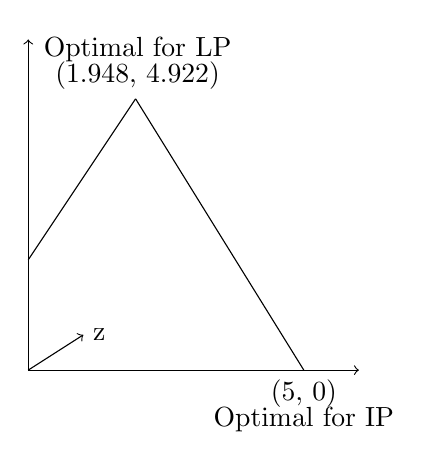
\begin{tikzpicture}[scale=0.7]
						\draw [->] (1,1) -- (1, 7);
						\draw [->] (1,1) -- (7, 1);
						\draw (1,3) -- (2.948, 5.922);
						\draw (2.948, 5.922) -- (6, 1);
						\draw [->] (1,1) -- (2, 1.64);
						\node [right] at (2, 1.64) {z};
						\node [above] at (2.984, 5.922) {(1.948, 4.922)};
						\node [above] at (2.984, 6.422) {Optimal for LP};
						\node [below] at (6,1) {(5, 0)};
						\node [below] at (6, 0.5) {Optimal for IP};
					\end{tikzpicture}
					\caption{Optimal solution for LP / IP}
				\end{figure}

			\subsection{Why Rounding Can be Bad - QAP example}
				Rounding can make the LP useless. For example, for QAP problem, the IP model is
				\begin{align}
					\text{min} \quad z &= \sum_{i\in D} \sum_{s\in O} c_is x_is + \sum_{i\in D} \sum_{j \in D} \sum_{s \in O} \sum_{t\in O} w_{ij}^{st}y_{ij}^{st}  \\
					\text{s.t.} \quad & \sum_{i \in D} x_{is} =1, \quad s\in D  \\
								&\sum_{s \in O} x_{is} = 1, \quad i \in D  \\
								&x_{is} \in \{0, 1\}, \quad i \in D, s\in O  \\
								& y_{ij}^{st} \ge x_{is} + x_{jt} - 1, \quad i\in D, j\in D, s\in O, t \in O  \\
								& y_{ij}^{st} \ge 0, \quad i\in D, j\in D, s\in O, t \in O  \\
								& y_{ij}^{st} \le x_{is}, \quad i\in D, j\in D, s\in O, t \in O  \\
								& y_{ij}^{st} \le x_{jt}, \quad i\in D, j\in D, s\in O, t \in O  
				\end{align}
				We can get the optimal solution for LP supposing $\forall i, s \quad x_{is}\in [0, 1]$
				\begin{align}
					x_{is} &= \frac{1}{|D|}, \quad i \in D, s\in O   \\
					y_{ij}^{st} & = 0, \quad i\in D, j\in D, s\in O, t \in O 
				\end{align}
				
			\subsection{IP and Convex Hull}
				For IP problem
				\begin{align}
					Z_{IP} \quad \text{max} \quad &z = cx  \\
							\text{s.t.} &Ax \le b \\
									&x\in {Z^n} 
				\end{align}
				In feasible region $S = \{x\in Z^n, Ax\le b\}$ , the optimal solution $Z_{IP} = \text{max}\{cx: x\in S\}$.\\
				Denote $conv(S)$ as the convex hull of $S$ then\\
				\begin{equation}Z_{IP}(S) = Z_{IP}(conv(S))  \end{equation}
				
			\subsection{Local Optimal and Global Optimal}
				Let 
				\begin{align}
					Z_s &= \text{min} \{f(x):x\in S\} \\
					Z_t &= \text{min} \{f(x):x\in T\}  \\
					& S \subset T 
				\end{align}
				then\\
				\begin{equation}Z_t \le Z_s  \end{equation}
				\textbf{Notice} that if $x_T^* \in S$ then $x_S^*=x_T^*$, to generalized it, \\
				We have
				\begin{align}
					\begin{cases}x_T^* \in \text{arg min} \{f(x): x\in T\} \\ x_T^* \in S\end{cases} \\ \Rightarrow x_T^*\in \text{arg min} \{f(x): x\in S\} 
				\end{align}
				Especially for IP, we can take the LP relaxation as $T$ and the original feasible region of IP as $S$, therefore, if we find an optimal solution from LP relaxation $T$ which is also a feasible solution of $S$, then it is the optimal solution for IP ($S$)
				
			\subsection{LP Relaxation}
				To perform the LP relaxation, we expand the feasible region
				\begin{align}
					x \in \{0,1\} & \rightarrow x\in [0, 1]  \\
					y\in Z^+ & \rightarrow y \ge 0 
				\end{align}
				If we have $Z_LP(s) = conv(s)$ then
				\begin{equation} LP(s): {x\in R_+^n: Ax\le b}\end{equation}
				The closer $LP(s)$ is to $conv(s)$ the better. Interestingly, we only need to know the convex in the direction of $c$.\\
				There are several formulation problem have the property of $Z_{LP}(s) = conv(s)$, such as:\\
				\indent- Assignment Problem\\
				\indent- Spawning Tree Problem\\
				\indent- Max Flow Problem\\
				\indent- Matching Problem

	\chapter{Decomposition Principle}

	\chapter{Ellipsoid Algorithm}

	\chapter{Projective Algorithm}

	\chapter{Interior-Point Algorithm}
	\part{Graph and Network Theory}
	\chapter{Basic concepts}
		\section{Graph}
			\begin{definition}[Graph]
				A \textbf{graph} G consists of a finite set $V(G)$ on vertices, a finite set $E(G)$ on edges and an \textbf{incident relation} than associates with any edge $e\in E(G)$ an unordered pair of vertices not necessarily distinct called \textbf{ends}.
			\end{definition}

			For example, the following graph\\
			\begin{figure}[!ht]
				\centering
				\begin{tikzpicture}[scale = 0.6, node distance = 1.7cm]
					\node (v_2) [circleNode] {$v_2$};
					\node (v_3) [circleNode, right of = v_2] {$v_3$};
					\node (v_1) [circleNode, below of = v_2] {$v_1$};
					\node (v_4) [circleNode, below of = v_3] {$v_4$};
					\node (v_5) [circleNode, right of = v_3] {$v_5$};
					\node (v_6) [circleNode, below of = v_5] {$v_6$};
					\draw [link] (v_2) -- node [left] {$e_2$} (v_1);
					\draw [link] (v_2) -- node [below] {$e_5$} (v_4);
					\draw [link] (v_1) to [out = 180, in = 270, looseness = 5] node [right] {$e_1$} (v_1);
					\draw [link] (v_2) to [out = 45, in = 135] node [above] {$e_3$} (v_3);
					\draw [link] (v_2) -- node [above] {$e_4$} (v_3);
					\draw [link] (v_3) -- node [right] {$e_6$} (v_1);
					\draw [link] (v_5) -- node [right] {$e_7$} (v_6);
				\end{tikzpicture}			
			\end{figure}\\
			can be represented as\\
			\begin{align}
				V = V(G) = \{v_1, v_2, v_3, v_4, v_5, v_6\} \\
				E = E(G) = \{e_1, e_2, e_3, e_4, e_5, e_6, e_7\}\\
				e_1 = v_1v_2, e_2 = v_2v_4, ...
			\end{align}

			\begin{definition}[loop, parallel, simple graph]
				An edge with identical ends is called a \textbf{loop}, Two edges having the same ends are said to be \textbf{parallel}, A graph without loops or parallel edges is called \textbf{simple graph}
			\end{definition}

			\begin{definition}[adjacent]
				Two edges of a graph are \textbf{adjacent} if they have a common end, two vertices are \textbf{adjacent} if they are jointed by an edge.
			\end{definition}

		\section{Subgraph}
			\begin{definition}[subgraph]
				Given two graphs $G$ and $H$, $H$ is a \textbf{subgraph} of $G$ if $V(H)\subseteq V(G)$, $E(H)\subseteq E(G)$ and an edge has the same ends in $H$ as it does in $G$. Furthermore, if $E(H)\neq E(G)$ then $H$ is a proper subgraph.
			\end{definition}
			
			\begin{definition}[spanning]
				A subgraph $H$ on $G$ is \textbf{spanning} if $V(H) = V(G)$
			\end{definition}

			\begin{definition}[vertex-induced, edge-induced]
				For a subset $V^{'}\subseteq V(G)$ we define an \textbf{vertex-induced} subgraph $G[V^{'}]$ to be the subgraph with vertices $V^{'}$ and those edges of $G$ having both ends in $V^{'}$. The \textbf{edge-induced} subgraph $G[E^{'}]$ has edges $E^{'}$ and those vertices of $G$ that are ends to edges in $E^{'}$.
			\end{definition}

			\notice{If we combine node-induced or edge-induced subgraphs $G(V^{'})$ and $G(V - V^{'})$, we cannot always get the entire graph.}

			\begin{definition}[degree]
				Let $v\in V(G)$, then the \textbf{degree} of $v\in V(G)$ denote by $d_G(v)$ is defines to be the number of edges incident of $v$. Loops counted twice.
			\end{definition}			

			\begin{problem}
				If $G$ is a simple graph with at least two vertices, prove that $G$ has two vertices with the same degree.
			\end{problem}

			\begin{proof}
				
			\end{proof}

			\begin{problem}
				Explain clearly, what is the largest possible number of vertices in a graph with 19 edges and all vertices of degree at least 3. Explain why this is the maximum value.
			\end{problem}

			\begin{theorem}
				For any graph $G=(V, E)$
				\begin{equation}
					\sum_{v\in V}d(v) = 2|E|
				\end{equation}			
			\end{theorem}

			\begin{proof}
				$\forall$ edge $e=\mu v$ with $\mu \neq v$, $e$ is  and counted once for $\mu$ and once for $v$, a total of two altogether. If $e=\mu \mu$, a loop, then it is counted twice for $\mu$			
			\end{proof}

			\begin{corollary}
				Every graph has an even number of odd degree vertices.
			\end{corollary}

			\begin{proof}
				\begin{equation}
					V = V_E\cup V_O \Rightarrow 
					\sum_{v\in V}d(v) = \sum_{v\in V_E} d(v) + \sum_{v\in V_O}d(v) = 2|E|
				\end {equation}			
			\end{proof}

	\chapter{Paths, Trees, and Cycles}
		\section{Walk}
			\begin{definition}[walk]
				A \textbf{walk} in a graph $G$ is a finite sequence $w=v_0e_1v_1e_2...e_kv_k$, where for each $e_i=v_{i-1}v_i$ the edge and its ends exists in $G$. We say that walk $v_0$ to $v_k$ on $(v_0, v_k)$-walk.
			\end{definition}

			\begin{example}
				\begin{equation}
					w = v_2e_4v_3e_4v_2e_5v_3
				\end{equation}
				is a walk, or $(v_2, v_3)$-walk				
			\end{example}

			\begin{definition}[origin, terminal, internal, length]
				For $(v_0, v_k)$-walk, The vertices $v_0$ and $v_k$ are called the \textbf{origin} and the \textbf{terminal} of the walk w, $v_1..v_{k-1}$ are called \textbf{internal} vertices. The integer $k$ is the \textbf{length} of the walk. Length of $w$ equals to the number of edges.
			\end{definition}
			
			We can create a reverse walk $w^{-1}$ by reversing $w$.
			\begin{equation}
				w^{-1} = v_ke_kv_{k-1}e_{k-1}...e_2v_1
			\end{equation}
			(The reverse walk is guaranteed to exist because it is an undirected graph)

			Given two walks $w$ and $w'$ we can create a third walk denoted by $ww'$ by concating $w$ and $w'$. The new walk's origin is the same as terminal.

		\section{Path and Cycle}
			\begin{definition}[trail]
				A \textbf{trail} is a walk with no repeating edges. e.g., $v_3e_4v_2e_5v_3$
			\end{definition}
			
			\begin{definition}[path]
				A \textbf{path} is a trail with no repeating vertices. e.g., $v_3e_4v_2$
			\end{definition}
			
			\notice{Paths $\subseteq$ Trails $\subseteq$ Walks}

			\begin{definition}[closed, cycle]
				A path is \textbf{closed} if it has positive length and its origin and terminal are the same. e.g., $v_1e_2v_2e_4v_3e_3v_1$. A closed trail where origin and internal vertices are distinct is called a \textbf{cycle} (The only time a vertex is repeated is the origin and terminal)
			\end{definition}
			
			\begin{definition}[even/odd cycle]
				A cycle is \textbf{even} if it has a even number of edges otherwise it is \textbf{odd}.
			\end{definition}

			\begin{problem}
				Prove that if $C_1$ and $C_2$ are cycles of a graph, then there exists cycles $K_1, K_2, ..., K_m$ such that $E(C_1)\Delta E(C_2) = E(K_1)\cup E(K_2) \cup...\cup E(K_m)$ and $E(K_i)\cap E(K_j)=\emptyset$. (For set $X$ and $Y$, $X\Delta Y = (X-Y)\cup(Y-X)$, and is called the symmetric difference of $X$ and $Y$)
			\end{problem}
			
			\begin{definition}[connected vertices]
				Two vertices $u$ and $v$ in a graph are said to be \textbf{connected} if there is a path between $u$ and $v$.
			\end{definition}
			
			\begin{definition}[component]
				Connectivity between vertices is an equivalence relation on $V(G)$, if $V_1, ... V_k$ are the corresponding equivalent classes then $G[V_1]...G[V_k]$ are \textbf{components} of G. If graph has only one component, then we say the graph is connected. A graph is connected iff every pair of vertices in G are connected, i.e., there exists a path between every pair of vertices.
			\end{definition}

		\section{Tree and forest}
			\begin{definition}[acyclic graph]
				A graph is called \textbf{acyclic} if it has no cycles
			\end{definition}
			
			\begin{definition}[forest, tree]
				A acyclic graph is called a \textbf{forest}. A connected forest is called a \textbf{tree}. 
			\end{definition}

			\begin{problem}
				Prove that if $T$ is a tree, then $T$ has exactly one more vertex than it has edges.
			\end{problem}

			\begin{proof}
				\begin{enumerate}
					\item For any tree $T$, there has to be at least one leaf, because a tree is acyclic and connected.
					\item Then, if we remove one leaf in the tree, i.e., we remove an edge and a vertex, where that vertex only connects to the edge we removed. One of the following situations will happen:
					\begin{enumerate}
						\item Situation 1: The remaining of $T$ is one vertex. In this case, $T$ has two vertices an one edge. (Exactly one more vertex than it has edges)
						\item Situation 2: The remaining of $T$ is another tree $T^{'}$ (removal of edges will not change acyclic), where $|V(T)| = |V(T^{'})| + 1$ and $|E(T)| = |E(V^{'}| + 1$. (one edge and one vertex has been removed)
					\end{enumerate}
					\item Do the leaf removal process recursively to $T^{'}$ if Situation 2 happens until Situation 1 happens. 
				\end{enumerate}
			\end{proof}

		\section{Spanning tree}
			\begin{definition}[spanning tree]
				A subgraph T of G is a \textbf{spanning tree} if it is spanning ($V(T)=V(G)$) and it is a tree.
			\end{definition}

			\begin{example}
				In the following graph\\
				\begin{figure}[!ht]
					\centering
					\begin{tikzpicture}[scale=0.6, node distance = 1.2cm]
						\node (v_2) [circleNode] {$v_2$};
						\node (v_3) [circleNode, right of = v_2] {$v_3$};
						\node (v_1) [circleNode, below of = v_2] {$v_1$};
						\node (v_4) [circleNode, below of = v_3] {$v_4$};
						\node (v_5) [circleNode, right of = v_3] {$v_5$};
						\draw [link] (v_1) -- (v_2);
						\draw [link] (v_2) -- (v_3);
						\draw [link] (v_1) -- (v_4);
						\draw [link] (v_2) -- (v_4);
						\draw [link] (v_3) -- (v_5);
						\draw [link] (v_4) -- (v_5);
						\draw [link] (v_1) -- (v_3);
					\end{tikzpicture}
				\end{figure}\\
				This is a spanning tree\\
				\begin{figure}[!ht]
					\centering
					\begin{tikzpicture}[scale=0.6, node distance = 1.2cm]
						\node (v_2) [circleNode] {$v_2$};
						\node (v_3) [circleNode, right of = v_2] {$v_3$};
						\node (v_1) [circleNode, below of = v_2] {$v_1$};
						\node (v_4) [circleNode, below of = v_3] {$v_4$};
						\node (v_5) [circleNode, right of = v_3] {$v_5$};
						\draw [link] (v_2) -- (v_3);
						\draw [link] (v_1) -- (v_4);
						\draw [link] (v_1) -- (v_3);
						\draw [link] (v_3) -- (v_5);
					\end{tikzpicture}
				\end{figure}
			\end{example}

			\begin{problem}
				Prove that if $T_1$ and $T_2$ are spanning trees of $G$ and $e\in E(T_1)$, then there exists a $f\in E(T_2)$, such that $T_1 - e + f$ and $T_2 + e - f$ are both spanning trees of $G$.
			\end{problem}

			\begin{proof}
				
			\end{proof}

			\begin{theorem}
				Every connected graph has a spanning tree.
			\end{theorem}			

			\begin{proof}
				Prove by constructing algorithm:
				\begin{algorithm}[!ht]
					\caption{Find a spanning tree for connected graph}
					\begin{algorithmic}[1]
						\REQUIRE a connected graph G and an enumeration $e_1,...e_m$ of the edges of G
						\ENSURE a spanning tree T of G
						\STATE Let T be the spanning subgraph of $G$ with $V(T)=V(G)$ and $E(T)=\emptyset$
						\STATE $i \gets 1$
						\WHILE {$i \le |E|$}
							\IF {$T + e_i$ is acyclic}
								\STATE $T \gets T + e_i$
								\STATE $i \gets i + 1$
							\ENDIF
						\ENDWHILE
					\end{algorithmic}
				\end{algorithm}				
			\end{proof}

			\notice{This algorithm can be improved, one idea is to make summation of edges in spanning subgraph less or equation to $|V| - 1$}

			For the complexity of spanning tree algorithm:
			\begin{enumerate}
				\item First we need to input the data, create an array such that the first and the second entries are the ends of $e_1$, third and fourth are the ends of $e_2$, and so on.
				\item The amount of storage needs in $2|E|$, which is $O(|E|)$
				\item The main work involved in the algorithm is for each edges $e_i$ and the current $T$, to determine if $T+e_i$ creates a cycle.
				\item At every stage $T$ has certain components $V_1, ... V_t$, (every time we add an edge, the number of components minus 1)
				\item So at the beginning $t = |V|$ with $|V_i| = 1 \forall i$
				\item At the end, $t = 1$
				\item suppose we keep each component $V_i$ by keeping for each vertex a pointer from the vertex to the name of the component containing it. Thus if $\mu \in V_3$, there will be a pointer from $\mu$ to integer 3.
				\item Then when edge $e_i = \mu v$ is enountered in Step 2, we see that $T+e_i$ contains a cycle if and only if $\mu$ and $v$ point to same integer which means they are in the same component
				\item If they are not in the same component, we want to add the edge which means then I have to update the pointers.
			\end{enumerate}

			To prove algorithm we need to show the output is a spanning tree, which means three properties must hold:
			\begin{itemize}
				\item spanning (Step I)
				\item acyclic (We never add an edge that create a cycle)
				\item connected (Proof by contradiction)
			\end{itemize}
			So it is sufficient to show that the output will be connected.
			\begin{proof}
				(Proof by Contradiction) Suppose the output graph $T$ of the algorithm is NOT connected. Let $T_1$ be a component of $T$, let $x\in T_1$ and $y \notin T_1$. But $G$ is a connected graph (given from the beginning), so there must be a path in $G$ that connects $x$ and $y$. Let such a path in $G$ be $p=xe_1v_1e_2,..v_{k-1}e_ky$. Clearly, $p\notin T_1$. So there must be a first vertex in $P$ that not in $T_1$. So $e_i \notin E(T)$, the only way this can happen when applying the algorithm is if $T + e_i$ creates a cycle $C$, i.e., $e_i \in C$, so $C - e_i$ is a path connecting $v_{i-1}$ and $v_i$. So $c - e_i \in T$, so $v_{i-1}$ is connected to $v_i \in T$. Contradiction. 
			\end{proof}

		\section{Special Graphs}
			\begin{definition}
				A \textbf{complete} graph $K_n (n \ge 1)$ is a simple graph with $n$ vertices and with exactly one edge between each pair of distinct vertices.
			\end{definition}

			\begin{definition}
				A \textbf{cycle} graph $C_n (n \ge 3)$ consists of $n$ vertices $v_1, ... v_n$ and $n$ edges $\{v_1, v_2\}, \{v_2, v_3\}, ... \{v_{n-1}, v_n\}$
			\end{definition}

			\begin{definition}
				A \textbf{wheel} graph $W_n (n \ge 3)$ is a simple graph obtains by adding one vertex to the cycle graph $C_n$, and connecting this new vertex to all vertices of $C_n$ 
			\end{definition}

			\begin{definition}
				A simple graph is said to be \textbf{bipartite} if the vertex set can be expressed as the union of two disjoint non-empty subsets $V_1$ and $V_2$ such that every edges has one end in $V_1$ and another end in $V_2$
			\end{definition}

			\begin{figure}[!ht]
				\centering
				\begin{tikzpicture}[node distance = 1.2cm]
					\node (A) [circleNode] {A};
					\node (B) [circleNode, right of = A] {B};
					\node (C) [circleNode, below of = A] {C};
					\node (D) [circleNode, right of = C] {D};
					\node (E) [circleNode, below of = C] {E};
					\node (F) [circleNode, right of = E] {F};
					\draw [link] (A) -- (B);
					\draw [link] (A) -- (D);
					\draw [link] (C) -- (B);
					\draw [link] (C) -- (F);
					\draw [link] (E) -- (D);
					\draw [link] (E) -- (F);
					\draw [link] (A) -- (F);
				\end{tikzpicture}
			\end{figure}

			\begin{definition}[complete bipartite]
				The \textbf{complete bipartite} graph $K_{mn}$ is the bipartite graph $V_1$ containing $m$ vertices and $V_2$ containing $n$ vertices such that each vertiex in $V_1$ is adjacent to every vertex in $V_2$
			\end{definition}

			\begin{example}
				Here is an example for $K_{53}$
				\begin{figure}[!ht]
					\centering
					\begin{tikzpicture}[node distance = 1.2cm]
						\node (A) [circleNode] {A};
						\node (B) [circleNode, below of = A] {B};
						\node (C) [circleNode, below of = B] {C};
						\node (D) [circleNode, below of = C] {D};
						\node (E) [circleNode, below of = D] {E};
						\node (F) [circleNode, right of = B] {F};
						\node (G) [circleNode, right of = C] {G};
						\node (H) [circleNode, right of = D] {H};
						\draw [link] (A) -- (F);
						\draw [link] (A) -- (G);
						\draw [link] (A) -- (H);
						\draw [link] (B) -- (F);
						\draw [link] (B) -- (G);
						\draw [link] (B) -- (H);
						\draw [link] (C) -- (F);
						\draw [link] (C) -- (G);
						\draw [link] (C) -- (H);
						\draw [link] (D) -- (F);
						\draw [link] (D) -- (G);
						\draw [link] (D) -- (H);
						\draw [link] (E) -- (F);
						\draw [link] (E) -- (G);
						\draw [link] (E) -- (H);
					\end{tikzpicture}
				\end{figure}
			\end{example}

			\begin{problem}
				Prove that a graph $G$ is bipartite iff every cycle is even.
			\end{problem}

		\section{Complexity}
			\fixme{This part is going to be moved to Algorithm notes (or I will just delete this part because of duplication).} We want to know guaranteed performances - "worse case" scenarios -  for any algorithm working on any problem instance.

			The following example is for addition of two matrices: \\
			\begin{algorithm}[!ht]
				\caption{Add two $m \times n$ matrices $A$, $B$ to get matrix $C$}
				\begin{algorithmic}
					\FOR {$i=1, 2, ..., m$}
						\FOR {$j=1, 2, ..., n$}
							\STATE $C_{ij} = A_{ij} + B_{ij}$
						\ENDFOR
					\ENDFOR
				\end{algorithmic}				
			\end{algorithm}\\

			The "running time" of an algorithm is measured by the number of basic operational steps.

			For so called "basic" steps, it includes
			\begin{itemize}
				\item $+$, $-$, $\times$, $\div$
				\item assignments and storage of a variable
				\item comparisons
			\end{itemize}

			For the example above
			\begin{itemize}
				\item $c_1 m n$ for addition $C_{ij} = A_{ij} + B_{ij}$
				\item $c_2 m n$ for saving $C_{ij}$
				\item $c_3 m n$ for comparison and assignment for $i$ and $j$
			\end{itemize}
			$c_1, c_2, c_3$ does not matter, the number of steps are $m \times n$, we say the algorithm runs $O(mn)$ (big O notation, the worse case)

			\begin{example}
				$f(n) = 3n^3 + 4n^2$\\
				Claim: $f(n)$ is $O(n^3)$\\
				Proof: Find a $c$ for $cn^3 - 3n^3 - 4n^2$ that there exist a $n_0$, for $\forall n \ge n_0$, the inequality holds.
			\end{example}

		\section{O notation, Omega notation, Theta notation}
			\begin{definition}[O notation]
				An algorithm is said to run in $O(f(n))$ time if for some constant $C (\ge 0)$, and $n_0$ the time takes algorithm is at most $Cf(n)$ for all $n\ge n_0$ 
			\end{definition}

			\begin{definition}[$\Omega$ notation]
				An algorithm is said to run in $\Omega(f(n))$ time if for some constant $C^{'} (\ge 0)$, and $n_0$. For all instance $n \ge n_0$, the time takes algorithm is at least $C^{'}f(n)$ for some instances. 
			\end{definition}

			\begin{definition}[$\Theta$ notation]
				An algorithm is said to be $\Theta(f(n))$ if it is both $O(f(n))$ and $\Omega(f(n))$
			\end{definition}

			\begin{example}
				$\frac{1}{2}n^2 - 3n$, $\Omega(n^2) \le \Theta(n^2) \le O(n^2)$\\
				Find $c^{'}$ and $c$ (both > 0) where $c^{'}n^2 \le \frac{1}{2}n^2 - 3n \le cn^2$ for a given $n_0$, $\forall n\ge n_0$ the inequality holds.\\
				Let $c^{'} = \frac{1}{14}$ and $c = \frac{1}{2}$, $\forall n \ge n_0$, where $n_0 = 7$, the inequality always holds.
			\end{example}

		\section{Representation of data}
			For set $\{1, 3, 4, 6, 8\}$ we have two ways to represent, array and list.

			For array, the representation is
			\begin{figure}[!ht]
				\centering
				\begin{tikzpicture}
					\matrix [rowArray] (rowArray) {
						1 & 2 & 3 & 4 & 5 & 6 & 7 & 8\\
						1 & 0 & 1 & 1 & 0 & 1 & 0 & 1\\
					};
				\end{tikzpicture}
			\end{figure}

			For list, the representation is
			\begin{figure}[!ht]
				\centering
				\begin{tikzpicture}[every node/.style = {rectangle split, rectangle split parts = 2, rectangle split horizontal}, node distance = 1em, start chain, every join/.style = {->, shorten <= -4.5pt}]
					\node [draw, on chain, join] {1};
					\node [draw, on chain, join] {3};
					\node [draw, on chain, join] {4};
					\node [draw, on chain, join] {6};
					\node [draw, on chain, join] {8};
				\end{tikzpicture}
			\end{figure}

			There is no "better" representation, one can be better than the other one in different cases.

			\begin{example}	
				For $\emptyset$, array need to build a space with $n$ cells of 0, complexity $O(n)$, list just need to build the first cell, $O(1)$
			\end{example}

			\begin{example}
				To find if a number is in a set, array needs $O(1)$ (look at the address), list needs $O(n)$ (loop through list, worst case, entire list)
			\end{example}

		\section{Size of a problem}
			Number of bits needed to store the problem

			\begin{example}
				Let $0 \le A_{ij} \le 2^{51}$
			\end{example}

			Representation by the bits of the number, $A_{ij} \le 2^51$ can be represented by max of $O(log(A_{ij}))$, (51 bits)

			For matrix addition that the total storage for addtion two matrix is $O(mnk)$, $k=O(log|A_{mn}|)$

	\chapter{Shortest-Path Problem}

	\chapter{Minimum Spanning Tree Problem}

	\chapter{Maximum Flow Problem}

	\chapter{Minimum Cost Flow Problem}

	\chapter{Assignment and Matching Problem}

	\chapter{Graph Algorithms}

	\chapter{Polygon Triangulation}
		\section{Types of Polygons}
			\begin{definition}[simple polygon]
				A \textbf{simple polygon} is a closed polygonal curve without self-intersection.
			\end{definition}

			\begin{figure}[h!]
				\centering
				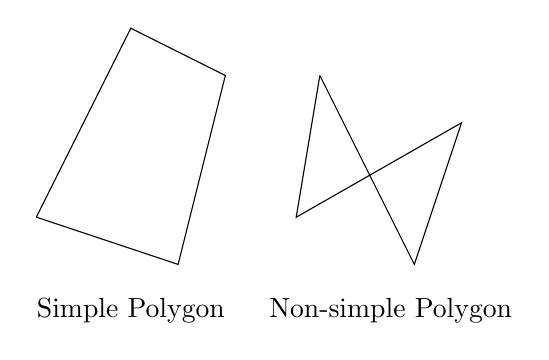
\begin{tikzpicture}[scale=0.6]
					\draw (0, 0) -- (3, -1) -- (4, 3) -- (2, 4) -- (0, 0);
					\draw (6, 3) -- (8, -1) -- (9, 2) -- (5.5, 0) -- (6, 3);
					\node at (2, -1.5) [below] {Simple Polygon};
					\node at (7.5, -1.5) [below] {Non-simple Polygon};
				\end{tikzpicture}
			\end{figure}

			Polygons are basic building blocks in most geometric applications. It can model arbitrarily complex shapes, and apply simple algorithms and algebraic representation/manipulation.
			
		\section{Triangulation}
			\begin{definition}[Triangulation]
				\textbf{Triangulation} is to partition polygon $P$ into non-overlapping triangles using diagonals only. It reduces complex shapes to collection of simpler shapes. Every simple $n$-gon admits a triangulation which has $n-2$ triangles.				
			\end{definition}

			\begin{figure}[h!]
				\centering
				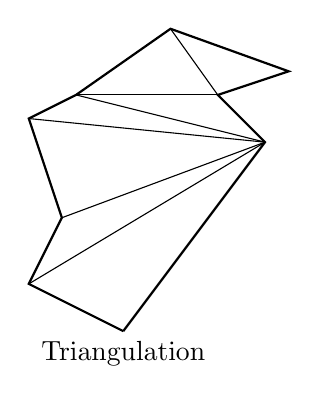
\begin{tikzpicture}[scale=0.6]
					\draw [thick] (0, 0) -- (3, 4) -- (2, 5) -- (3.5, 5.5) -- (1, 6.4) -- (-1, 5) -- (-2, 4.5) -- (-1.3, 2.4) -- (-2, 1) -- (0, 0);
					\draw (-2, 1) -- (3, 4);
					\draw (-1.3, 2.4) -- (3, 4);
					\draw (-2, 4.5) -- (3, 4);
					\draw (-1, 5) -- (3, 4);
					\draw (-1, 5) -- (2, 5);
					\draw (2, 5) -- (1, 6.4);
					\node at (0, 0) [below] {Triangulation};
				\end{tikzpicture}
			\end{figure}

			\begin{theorem}
				Every polygon has a triangulation				
			\end{theorem}

			\begin{lemma}
				Every polygon with more than three vertices has a diagonal.
			\end{lemma}

			\begin{proof}
				(by Meisters, 1975) Let $P$ be a polygon with more than three vertices. Every vertex of a $P$ is either \textit{convex} or \textit{concave}. W.L.O.G.(any polygon must has convex corner) Assume $p$ is a convex vertex. Denote the neighbors of $p$ as $q$ and $r$. If $\bar{qr}$ is a diagonal, done, and we call $\triangle{pqr}$ is an \textit{ear}. If $\triangle{pqr}$ is not an ear, it means at least one vertex is inside $\triangle{pqr}$, assume among those vertexes inside $\triangle{pqr}$, $s$ is a vertex closest to $p$, then $\bar{ps}$ is a diagonal.
			\end{proof}
			
		\section{Art Gallery Theorem}
			\begin{theorem}
				Every $n$-gon can be guarded with $\lfloor \frac{n}{3} \rfloor$ vertex guards
			\end{theorem}

			\begin{lemma}
				Triangulation graph can be 3-colored.
			\end{lemma}

			\begin{problem}
				The floor plan of an art gallery modeled as a simple polygon with $n$ vertices, there are guards which is stationed at fixed positions with 360 degree vision but cannot see through the walls. How many guards does the art gallery need for the security? (Fun fact: This problem was posted to Vasek Chvatal by Victor Klee in 1973).				
			\end{problem}

			\begin{proof}
				- $P$ plus triangulation is a planar graph\\
				- 3-coloring means there exist a 3-partition for vertices that no edge or diagonal has both endpoints within the same set of vertices.\\
				- Proof by Induction:\\
				\indent - Remove an ear (there will always exist ear) \\
				\indent - Inductively 3-color the rest\\
				\indent - Put ear back, coloring new vertex with the label not used by the boundary diagonal.
			\end{proof}

		\section{Triangulation Algorithms}

		\section{Shortest Path}



	\part{Integer and Combinatorial Programming}
	\chapter{Formulation}
		\section{Typical Problems}

		\section{Integer Programming Formulation Skills}
			\subsection{A Variable Taking Discontinuous Values}
				\framebox{\textbf{Description:}} In algebraic notation: 
				\begin{equation}
					x = 0,\quad \text{or} \quad l\le x \le u \nonumber
				\end{equation}
				\framebox{\textbf{Modeling:}}
				\begin{align}
					& x \le uy\nonumber \\
					& x \ge ly \nonumber \\
					& y \in \{0, 1\} \nonumber
				\end{align}
				where
				\begin{equation}y=\begin{cases}0, & \text{if }x=0 \\ 1, & \text{if } l\le x \le u\end{cases}\nonumber \end{equation}
					
			\subsection{Fixed Costs}
				\framebox{\textbf{Description:}} In algebraic notation: 
				\begin{equation}
					C(x) = \begin{cases} 0 & \text{for } x=0 \\ k + cx & \text{for } x > 0 \end{cases} \nonumber
				\end{equation}
				\framebox{\textbf{Modeling:}}
				\begin{align}
					& C^*(x, y) = ky+cx\nonumber\\
					& x \le My \nonumber \\
					& x \ge 0 \nonumber\\
					& y \in \{0, 1\} \nonumber
				\end{align}
				where
				\begin{equation}y=\begin{cases}0, & \text{if }x=0 \\ 1, & \text{if }x\ge 0\end{cases}\nonumber \end{equation}
			
			\subsection{Either-or Constraints}
				\framebox{\textbf{Description:}} In algebraic notation: 
				\begin{equation}
					\sum_{j\in J} a_{1j} x_j \le b_1 \text{ or } \sum_{j\in J} a_{2j} x_j \le b_2 \nonumber
				\end{equation}
				\framebox{\textbf{Modeling:}}
				\begin{align}
					& \sum_{j\in J} a_{1j} x_j \le b_1 + M_1y \nonumber \\
					& \sum_{j\in J} a_{2j} x_j \le b_2 + M_1(1-y) \nonumber \\
					& y \in \{0, 1\} \nonumber
				\end{align}
				where
				\begin{equation}y=\begin{cases}0, & \text{if }\sum_{j\in J} a_{1j} x_j \le b_1 \\ 1, & \text{if } \sum_{j\in J} a_{2j} x_j \le b_2\end{cases}\nonumber \end{equation}
				Notice that the sign before $M$ is determined by the inequality $\ge$ or $\le$, if it is \lq\lq{}$\ge$\rq\rq{}, use \lq\lq{}$-$\rq\rq{}, if it \lq\lq{}$\le$\rq\rq{}, use \lq\lq{}+\rq\rq{}.
			
			\subsection{Conditional Constraints}
				\framebox{\textbf{Description:}} If constraint A is satisfied, then constraint B must also be satisfied
				\begin{equation}
					\text{If} \quad \sum_{j\in J} a_{1j} x_j \le b_1 \text{ then } \sum_{j\in J} a_{2j} x_j \le b_2 \nonumber
				\end{equation}
				The key part is to find the opposite of the first condition. We are using $A\Rightarrow B \Leftrightarrow \neg B \Rightarrow \neg A$\\
				Therefore it is equivalent to
				\begin{equation}
					\sum_{j\in J} a_{1j} x_j > b_1 \text{ or } \sum_{j\in J} a_{2j} x_j \le b_2 \nonumber
				\end{equation}
				Furthermore, it is equivalent to
				\begin{equation}
					\sum_{j\in J} a_{1j} x_j \ge b_1 + \epsilon \text{ or } \sum_{j\in J} a_{2j} x_j \le b_2 \nonumber
				\end{equation}
				Where $\epsilon$ is a very small positive number.\\
				\framebox{\textbf{Modeling:}}
				\begin{align}
					& \sum_{j\in J} a_{1j} x_j \ge b_1 + \epsilon -  M_2y \nonumber \\
					& \sum_{j\in J} a_{2j} x_j \le b_2 + M_2(1-y) \nonumber \\
					& y \in \{0, 1\} \nonumber
				\end{align}	
			
			\subsection{Special Ordered Sets}
				\framebox{\textbf{SOS1 Description}} Out of a set of yes-no decisions, at most one decision variable can be yes. \
				\begin{align}
					x_1=1,x_2=x_3&=\dots=x_n=0 \nonumber \\
					&\text{or} \nonumber \\
					x_2=1, x_1=x_3&=\dots=x_n=0 \nonumber \\
					&\text{or ...} \nonumber
				\end{align} 
				\framebox{\textbf{Modeling:}}
				\begin{equation} \sum_{i} x_i = 1, \quad i \in N\nonumber \end{equation}
				\framebox{\textbf{SOS2 Description 1}} Out of a set of binary variables, at most two variables can be nonzero. In addition, the two variables must be adjacent to each other in a fixed order list.\\
				\framebox{\textbf{Modeling:}}
				If $x_1, x_2, ... , x_n$ is a SOS2, then
				\begin{align}
					& \sum_{i=1}^{n} x_i \le 2 \nonumber \\
					& x_i + x_j \le 1, \forall i \in \{1, 2,..., n\}, j \in \{i+2, i+3, ..., n\} \nonumber \\
					&x_i \in \{0, 1\}\nonumber
				\end{align}
				\framebox{\textbf{SOS2 Description 2}} There is another type of definition, that is out of a set of nonnegative variables \textbf{not binary here}, at most two variables can be nonzero. In addition, the two variables must be adjacent to each other in a fixed order list. All variables summing to 1.\\
				This definition of SOS2 is used in the following section \textit{Piecewise Linear Formulations}\\
								
			\subsection{Piecewise Linear Formulations}
				\framebox{\textbf{Description:}} The objective function is a sequence of line segments, e.g. $y=f(x), $ consists $k-1$ linear segments going through $k$ given points $(x_1, y_1), (x_2, y_2), ... ,(x_k, y_k)$.\\
				Denote 
				\begin{equation}d_i=\begin{cases}1, & x\in (x_i, x_{i+1})\\0, & \text{otherwise} \end{cases}\nonumber\end{equation}
				Then the objective function is
				\begin{equation}\sum_{i \in \{1, 2, ..., k-1\}} y = d_if_i(x)\nonumber \end{equation} 
				\framebox{\textbf{Modeling:}} Given that objective function as a piecewise linear formulation, we can have these constraints\\
				\begin{align}
					&\sum_{i \in \{1, 2, ..., k-1\}} d_i =1 \nonumber \\
					&d_i \in \{0, 1\}, i \in \{1, 2, ..., k-1\} \nonumber \\
					& x = \sum_{i \in \{1, 2, ..., k\}} w_i x_i \nonumber \\
					& y = \sum_{i \in \{1, 2, ..., k\}} w_i y_i \nonumber \\
					& w_1 \le d_1 \nonumber \\
					& w_i \le d_{i-1} + d{i}, i \in \{2, 3, ..., k-1\} \nonumber \\
					& w_k \le d_{k-1} \nonumber
				\end{align}
				In this case, $ w_i \in SOS2$ (second definition)		
									
			\subsection{Conditional Binary Variables}
				\framebox{\textbf{Description:}} Choose at most $n$ binary variable to be 1 out of  $x_1, x_2, ... x_m, m\ge n$. If $n=1$ then it is SOS1.\\
				\framebox{\textbf{Modeling:}}
				\begin{equation}
					\sum_{k\in \{1,2,...,m\}} x_k \le n\nonumber
				\end{equation}
				\framebox{\textbf{Description:}} Choose exactly $n$ binary variable to be 1 out of  $x_1, x_2, ... x_m, m\ge n$\\
				\framebox{\textbf{Modeling:}}
				\begin{equation}
					\sum_{k\in \{1,2,...,m\}} x_k = n\nonumber
				\end{equation}
				\framebox{\textbf{Description:}} Choose $x_j$ only if $x_k = 1$\\
				\framebox{\textbf{Modeling:}}
				\begin{equation}x_j = x_k \nonumber \end{equation}
				\framebox{\textbf{Description:}} \lq\lq{}and\rq\rq{} condition, iff $x_1, x_2, ... , x_m =1$ then $y=1$\\
				\framebox{\textbf{Modeling:}}
				\begin{align}
					& y \le x_i, i\in \{1, 2, ..., m\} \nonumber \\
					& y \ge \sum_{i \in \{1, 2, ..., m\}} x_i - (m - 1) \nonumber
				\end{align}

			\subsection{Elimination of Products of Variables}
				\framebox{\textbf{Description:}} For variables $x_1$ and $x_2$,
				\begin{equation}y = x_1 x_2\nonumber\end{equation}
				\framebox{\textbf{Modeling:}} If $x_1, x_2$ are binary, it is the same as \lq\lq{}and\rq\rq{} condition of binary variables.\\
				If $x_1$ is binary, while $x_2$ is continuous and $0 \le x_2 \le u$, then
				\begin{align}
					y &\le ux_1 \nonumber \\
					y &\le x_2 \nonumber \\
					y &\ge x_2 - u(1- x_1) \nonumber \\
					y &\ge 0 \nonumber
				\end{align}
				If both $x_1$ and $x_2$ are continuous, it is non-linear, we can use Piecewise linear formulation to simulate.

	\chapter{Branch and Bound}

	\chapter{Branch and Cut}

	\chapter{Packing and Matching}

	\chapter{Traveling Salesman Problem}

	\chapter{Knapsack Problem}
	\part{Nonlinear Programming}
	\chapter{Introduction and Movtivation}
		\section{Basic concept}
			\begin{align}
				\min \quad &f(x) \\
				\text{s.t.} \quad & g_i(x) \le 0, \quad \forall i = 1, ..., m\\
								  & h_i(x) = 0, \quad \forall i = 1, ..., m\\
								  &x \in X
			\end{align}

			Iso-value curve\\
			Given a function $f(x): R^n \rightarrow R$, the iso-value curve of level k, denoted by $L_k$ is the set of points for which $f(x)=k$, Formally,
			\begin{equation}
				L_k = \{x \in R^n | f(x)=k\}
			\end{equation}

			Observations:\\
			\indent - An optimization problem may not have a feasible solution\\
			\indent - Even if the problem has a feasible solution, the problem may not have an optimal solution\\
			\indent - If an optimal solution exists, then\\
			\indent \indent - if may be unique
			\indent \indent - it may be a convex set
			\indent \indent - it may be serveral sets

			The following two problems are equivalent
			\begin{align}
				\min \quad & x_1 + x_2\\
				\text{s.t.} \quad & x_1 + 2x_2\le 3 \\
				                  & x_1, x_2 \in \{0, 1\}
			\end{align}
			and 
			\begin{align}
				\min \quad & x_1 + x_2\\
				\text{s.t.} \quad & x_1 + 2x_2\le 3 \\
				                  & x_1 \ge 0 \\
				                  & x_2 \ge 0 \\
				                  & x_1(1 - x_1) = 0\\
				                  & x_2(1 - x_2) = 0
			\end{align}		

			\section{Example - Braess Paradox}

			- Situation 1, minimizing total time
			\begin{align}
				\min \quad & \frac{x_1t_1 + x_2t_2 + x_3t_3}{x_1 + x_2 + x_3}\\
				\text{s.t.} \quad & x_1 + x_2 + x_3 = 1000\\
				                  & t_1 = 1 + (x_1 + x_2) / 1000 + 2\\
				                  & t_2 = 1 + (x_1 + x_2) / 1000 + 0.25 + (x_2 + x_3)/1000 + 1\\
				                  & t_3 = 2 + (x_2 + x_3) / 1000 + 1
			\end{align}

			- Situation 2, selfish for driver
			\begin{align}
				\text{s.t.} \quad & x_1 + x_2 + x_3 = 1000\\
				                  & t_1 = 1 + (x_1 + x_2) / 1000 + 2\\
				                  & t_2 = 1 + (x_1 + x_2) / 1000 + 0.25 + (x_2 + x_3)/1000 + 1\\
				                  & t_3 = 2 + (x_2 + x_3) / 1000 + 1\\
				                  & x_1 t_1 \le x_1 t_2 \\
				                  & x_1 t_1 \le x_1 t_3 \\
				                  & x_2 t_2 \le x_2 t_1 \\
				                  & x_2 t_2 \le x_2 t_3 \\
				                  & x_3 t_3 \le x_3 t_1 \\
				                  & x_3 t_3 \le x_3 t_2
			\end{align}

			- Situation 3, remove one of the arc, remove $x_2$ and all related constraints

		\section{Newsvendor problem}
			Parameter
			\begin{itemize}
				\item for each newspaper, cost is \$c
				\item vendor determine the number of newspaper to buy as $N$
				\item each news paper selled for \$p
				\item each news paper has a salvage value of \$v
				\item for demend scenario $d_i, i\in N$, the probability is $\pi_i \in N$
			\end{itemize}

			Decision Vars
			\begin{itemize}
				\item number of newspaper to buy, $q$
				\item number of newspaper returned, $r_i, i \in N$
				\item number of newspaper sold, $s_i, i\in N$
			\end{itemize}

			Constraints
			\begin{itemize}
				\item $q = s_i + r_i$
				\item $s_i = \min \{d_i, q\}$
				\item $q \in Z_+ \cup \{0\}$
				\item $r_i, s_i \in Z_+ \cup \{0\}$
			\end{itemize}

			Objective Fuction
			\begin{equation}
				\max \quad \sum_{i \in N} \pi_i (ps_i + vr_i) - cq
			\end{equation}

		\section{Portfolio optimization}
			Parameters
			\begin{itemize}
				\item A, set of assets
				\item $\bar{r}$, desired portfolio's return
				\item $r_i$, expected return of $i\in A$
				\item $\sigma_{ij}^2$, covariance between $i$ and $j$, $i, j \in A$
			\end{itemize}

			Decision Vars
			\begin{itemize}
				\item $x_i$ \% of total budget to invest to asset $i \in A$
			\end{itemize}

			Constraints
			\begin{itemize}
				\item $\sum_{i \in A} x_i = 1$
				\item $\sum_{i \in A} \alpha_i x_i \ge \bar{r}$
				\item Nonnegativity
			\end{itemize}

			Objective function
			\begin{equation}
				\min \quad \sum_{i \in A}\sum_{j \in A} \sigma_{ij}^2 x_i x_j
			\end{equation}

		\section{curve fitting}
			
	\chapter{Background}
		\section{Operations}
			A vector addition $\oplus$ has such feature
			\begin{itemize}
				\item $\oplus$ is closed
				\item $\oplus$ is commutative
				\item $\oplus$ is associative
				\item $\oplus$ has an identity element
				\item $\oplus$ has an inverse
			\end{itemize}

			A scalar multiplication $\otimes$ has the following features
			\begin{itemize}
				\item $\otimes$ is closed
				\item $\otimes$ is distributive wrt $\oplus$
				\item $\otimes$ is distributive wrt scalar addition, i.e. $(\lambda + \mu) \otimes v = (\lambda \otimes v) \oplus (\mu \otimes v$
				\item $\otimes$ is distributive with multiplication
			\end{itemize}

			\begin{equation}
				u \oplus v = \left[\begin{align}u_1 \\ u_1\end{align}\right] \oplus \left[\begin{align}v_1 \\ v_1\end{align}\right]
			\end{equation}

			For $W_1 = \{w \in R^3 | 3w_1 + 2w_2 + w_3 = 0\}$
			Check if this is closed to $\oplus$

			\begin{align}
				a, b &\in W_1 \\
				3a_1 + 2a_2 + a_3 & = 0\\
				3b_1 + 2b_2 + b_3 & = 0\\
				c & = a + b
				c & = 3 (a_1 + b_1) + ... = 0
			\end{align}

	\chapter{KKT Optimality Conditions}

	\chapter{Lagrangian Duality}

	\chapter{Unconstrained Optimization}

	\chapter{Penalty and Barrier Functions}
	\part{Algorithms and Computational Complexity}
	\chapter{Computational Complexity}

	\chapter{Sorting}
		\section{Elementary Sorting Algorithms}

		\section{Heap-sort}

		\section{Quick-sort}

		\section{Sorting in Linear Time}

		\section{Medians and Order Statistics}

	\chapter{Data Structures}
		\section{Elementary Data Structures}

		\section{Hash Tables}

		\section{Binary Search Trees}

		\section{Red-Black Trees}

		\section{B-Trees}

		\section{Fibonacci Heaps}

		\section{van Emde Boas Trees}

	\chapter{Design and Analysis Techniques}
		\section{Dynamic Programming}

		\section{Greedy Algorithms}

		\section{Amortized Analysis}

		\section{Multi-threaded Algorithms}

		\section{Matrix Operations}

		\section{Polynomials and the FFT}

		\section{Number-Theoretic Algorithms}

		\section{String Matching}

		\section{Computational Geometry}

		\section{NP-Completeness}

		\section{Approximation Algorithms}

	\part{Heuristics ans Meta-heuristics}
	\include{07-Game_Theory}
	\include{08-Probability_Stochastic_Process_and_Markov_Chains}
	\include{09-Queuing_Theory}
	\include{10-Inventory_Theory}
	\include{11-Reliability_Theory}
	\include{12-Statistic}
	\include{13-Simulation}
\end{document}